\section{Discussion and Results}
\label{chap:Discussion and Results}

\subsection{Handling the raw data and choosing a security}
\label{chap:Handling the raw data and choosing a security}

\quad Our raw data came from B3 Brazilian's stock exchange, which can be download freely from \href{http://www.b3.com.br/pt_br/market-data-e-indices/servicos-de-dados/market-data/cotacoes/cotacoes/}{its website}. The files contain all negotiations (historical series of data) for all securities from a trading section (day). We have downloaded the files containing the data-series from 22.06.2020 to 04.12.2020, and the chosen security that our studies will focus on will be PETR4. For that, a python function called get\_instrument() in the \href{https://github.com/fabiorodp/UiO-FYS-STK4155/tree/master/Project3/package/read_data.py}{Project3/package/read\_data.py} file does the job of extracting all negotiations for PETR4.\\

It is essential to state that PETR4 is the biggest specialized company in Brazil's oil, natural gas, and energy industry. Besides, in the B3 market, this stock has one of the highest liquidity flow that guarantee us to avoid higher price gaps, slippage, or any other trading issues. These reasons justify our choice for PETR4, but any additional security can perform the following experiments.

\subsection{Engineering the features and deciding the prediction's targets}
\label{chap:Engineering the features and deciding the prediction's targets}

\quad Most of the studies using ANN for time series forecasting uses input data holding the stock daily (OLHC) opening, lowest, highest, and closing prices \hyperref[Bib:Leonardo C. Martinez, Diego N. da Hora, Joao R. de M. Palotti, Wagner Meira Jr. and Gisele L. Pappa]{[5]}\hyperref[Bib:Van-Dai Ta, Chuan-Ming Liu, Direselign Addis Tadesse]{[6]}[9]. The input may include many other \hyperref[chap:Technical Analysis]{technical analysis (TA)} or fundamental analysis (FA) indicators.\\

As this report considers short-term trading structures, there is no reason to use fundamentalists' indicators published quarterly. However, technical indicators are very relevant and useful to bring more information to our ANN's models. Hence, as introduced in the theory section of this work, we will use three technical tools, such that, \hyperref[chap:Simple Moving Average (SMA)]{Simple Moving Average (SMA)}, \hyperref[chap:Exponential Moving Average (EMA)]{Exponential Moving Average (EMA)}, and \hyperref[chap:Bollinger Bands (BB)]{Bollinger Bands (BBs)}.\\

Therefore, the 16 variables/features used as input to RNN and LSTM are described in the following list:

\begin{itemize}
\item 4 features containing the opening, lowest, highest, closing prices and volume (OLHCV);
\item 9 features containing the upper, middle and lower BBs for 5, 10 and 20 periods;
\item 3 features containing the EMAs for 5, 10 and 20 periods;
\end{itemize}

Remark that these features test the ability of the RNN and LSTM to learn from previous information of the time series data. Besides, these features were chosen according to the author's trading practices, but it could have been chosen in any other preferable periods. As a future research objective, it would be a relevant idea to study the effect of several indicators in the learning and the appropriate amount of historical data that should be considered.\\

Regarding the prediction's targets, we want to design a valuable tool for algorithm tradings and decision-making processes. The idea is to predict the highest and lowest of the next trading section (next day). This information would bring a rouge advance and benefit for day-traders because they will start the day already knowing the probable highest and lowest and, consequently, avoid trading operations in the wrong direction against the oversold (lowest of the day) overbought (highest of the day) areas.

\subsection{Time series Cross-Validation}
\label{chap:Time series Cross-Validation}

\quad The Machine Learning system, in general, learns the data's structure so that we can predict the future. When we fit and train the learning algorithm, it does not surprise the spectacular results that can be found. Still, it typically has zero forecasting power if not tested with unseen data \hyperref[Bib:Lopez de Prado]{[4][p. 131]}. Therefore, one solution is to perform Cross-Validation (CV) splits, where we separate the entire data on training and testing sets.\\

Regarding time-series data, the typical CV, which handles independent identically distributed (IID) sets, fails in its proposes. Indeed, we are dealing with ordered, recurrent, and serially-correlated data, which can not be split into unordered blocks or even shuffled. Besides, it is also common to have leakage \hyperref[Bib:Lopez de Prado]{[4][p. 131]} when pieces of information from the training set also arise in the testing sets. One widespread example of leakage is when one wants to predict a period's closing price giving the highest and lowest of the same time step. The ideal in this scenario is to provide the highest and lowest of the previous time step. Thinking on leakage, Professor Marcos Lopes de Prado elaborated a policy to reduce the likelihood of leakage, \textit{ipsis verbis} \hyperref[Bib:Lopez de Prado]{[4][p. 132]}:\\

\noindent \textit{\textbf{1st.} Drop from the training set any observation $i$ where $Y_i$ is a function of information used to determine $Y_j$, and $j$ belongs to the testing set.}\\

\qquad \textit{\textbf{(a)} For examples, $Y_i$ and $Y_j$ should not span overlapping periods.}\\

\noindent \textit{\textbf{2nd.} Avoid over-fitting the classifier. In this way, even if some leakage occurs, the classifier will not be able to profit from it. Use:}\\

\qquad \textit{\textbf{(a)} Early stopping of the base estimators;}\\

\qquad \textit{\textbf{(b)} Bagging of classifiers, while controlling for oversampling on redundant examples, so that the individual classifiers are as diverse as possible.}\\

\qquad \qquad \textit{\textbf{(b.i)} Set max\_samples to the average uniqueness.}\\

\qquad \qquad \textit{\textbf{(b.ii)} Apply sequential bootstrap.}\\

In this project, we have followed Prado's policies for avoiding leakages.\\

For the CV technique, we have used the proposed methodology given by \hyperref[Bib:Hyndman, R.J., and Athanasopoulos, G.]{[9]}[\href{https://otexts.com/fpp2/}{Ch.3.4}], which describes a procedure for testing unseen data with series of test sets containing a single observation, and the corresponding training set consists of rolled samples that occurred before. The diagram that illustrates the series of training and testing sets follows \hyperref[Bib:Hyndman, R.J., and Athanasopoulos, G.]{[9][Ch.3.4]}:

\begin{figure}[H]
\label{fig:CV}
\centering
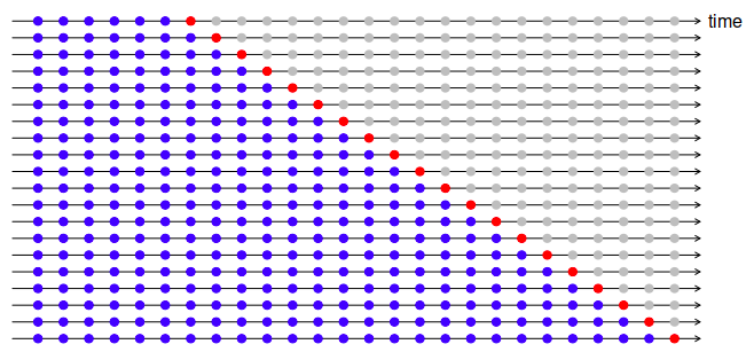
\includegraphics[height=4cm]{CV}
\caption{Time series CV using \textit{"evaluation on a rolling forecasting origin"}\hyperref[Bib:Hyndman, R.J., and Athanasopoulos, G.]{[9][Ch.3.4]}}
\end{figure}

The accuracy of the predictions will be calculated by averaging over the Mean Squared Error (MSE) and Mean Absolute Error (MAE) resulted from all training and validations. This method is called \textit{"evaluation on a rolling forecasting origin"} by the authors \hyperref[Bib:Hyndman, R.J., and Athanasopoulos, G.]{[9][Ch.3.4]} because of the training sets based on rolls ahead in time.\\

Our script called studies.py in Project3/package/ directory performs a Time series Cross-Validation with parameter combination of Units and Epochs. The beginning's rolling value for training is defined by default as 60-time steps, which means that our ANN model will start the training with the first 60-days of data, and then it validates the 61's day and measure the testing metrics. The CV algorithm keeps doing the same procedure for the next steps, training 61-days and validating the 62's day, until all data have been gone. In the end, the average testing metrics are returned for an assessment of the best model and parameters.

\subsection{Training RNN model and optimizing hyper-parameters}
\label{chap:Training RNN model and optimizing hyper-parameters}




\subsection{Training LSTM model and optimizing hyper-parameters}
\label{chap:Training LSTM model and optimizing hyper-parameters}

\subsection{Applying the predictions to an algorithm trading strategy}
\label{chap:Applying the predictions to an algorithm trading strategy}
